\documentclass[12pt, a4paper, twocolumn] {article} % Define a estrutura base do documento, tamanho da fonte, papel e disposição de colunas
\usepackage[brazilian]{babel} % Traduz padrões e regras de hifenização
\usepackage[utf8]{inputenc} % Habilita digitação de acentos no editor
\usepackage[T1]{fontenc} % 
\usepackage{lipsum} %Biblioteca de lero lero
\usepackage[
    top=3cm,
    left=3cm,
    bottom=2cm,
    right=2cm
]{geometry} % Seta as margens
\usepackage{setspace}
\usepackage{enumitem} %lista numerada
\usepackage{graphicx} %habilita imagem
\usepackage{booktabs} %tabelas de alto nível


%\onehalfspacing % Habilita espaçamento entre linhas
\setlength{\parindent}{1.25cm} % Indentação a partir do segundo parágrafo

\title{Isto é um projeto \LaTeX} % Define o título do documento

\author % Elenca os autores do projeto
    {KALEBE SCHEIDT\thanks{UDESC - kalebe.scheidt@edu.udesc.br}}
    
\date{\today} % Insere a data atual no documento

\begin{document} % Abre o corpo do texto

\maketitle % Printa o título na tela

\begin{abstract} % Abre o campo resumo
    \lipsum[1-2] % Enche o resumo de lixo
\end{abstract} % Fecha o campo resumo


\tableofcontents % Sumário, mas é só pra saber como faz mesmo

\section{Introdução} % Cria sessão
Seja bem-vindo. A serventia primária do presente documento é convir ao seu autor tal qual o diário de Ismael em Moby Dick\footnote{Livro grande sobre uma baleia maior ainda, famoso pelas suas enrolações e história com o desfecho mais óbvio da literatura mundial.}, isto é, um registro do andamento do curso de LaTeX. Contudo, a ideia não é ser uma sítense do curso \textit{per se}, mas sim uma documentação aplicada na prática.


A estrutura base do documento é separada de acordo com o número de aulas do curso, conforme já é possível conluir ao conferir o sumário. Cada capítulo toma forma de acordo com as novas habilidades adquiridas, bem como o restante do documento sofre uma estilização padronizada e vai caminhando em rumo à \textbf{perfeição}\footnote{Característica do que é perfeito.}.

\section{Fundamentação Teórica}

Este tópico serve para descrever de forma teórica o conteúdo técnico a ser abordado nas aulas, mantendo uma linguagem acessível, mas eventualmente confuda por se tratar da compreensão do autor, algo que não reflete com exatidão a documentação oficial.

\subsection{Formatação Textual e Pacote Geometry}
Como tudo na vida, existem regras até mesmo para as margens de um documento científico. Nesse aspecto, o pacote geometry é um salvador no mundo do \LaTeX. Com ele é possível alterar as dimensões das margens nos mínimos detalhes, algo bastante útil para lidar com as regras, por vezes diferenciadas, da ABNT\footnote{Associação Brasileira de Normas Técnicas. Como é de se esperar, nada disso presta pra nada no mundo fora do Brasil, então aproveite com moderação.}.


No que diz respeito à formatação textual, existem diferenças expressivas entre fazer isso no Word\footnote{Treco da Microslop que nunca mais será utilizado pelo presente autor para edição de texto.}, por exemplo, ou em \LaTeX. No primeiro, a estilização textual ocorre de forma visual, tal qual todas as demais configurações no ambiente deles. Já no LaTeX, tal estilização acontece puramente dentro do próprio bloco de texto, seguindo a estrutura padrão de comandos. Pode parecer complexo em um primeiro momento, mas a beleza do processo compensa a curva de aprendizado.

\subsection{O Paradigma LaTeX} % Cria subsessão
Quando falamos sobre a criação da tecnologia, houve um conflito muito interessante entre duas vertentes de pensamento chamaadas de: \textbf{WYSIWYG e WYSIWYM}. A primeira trabalha a abordagem de \textit{What You See Is What You Get}, ou seja, o que você está vendo é exatamente como o documento vai ficar nos finalmentes, focando exclusivamente na abordagem visual. Vários softwares de edição de texto trabalham dessa forma, tais como \textbf{Microsoft Office; LibreOffice.} No segundo caso, o foco está no que o usuário \textbf{quer dizer}, por esse motivo o significado da sigla é \textit{What You See Is What You Mean}, focando em uma abordagem focada no \textit{feeling} do usuário. Pode parecer confuso, mas vai fazer sentido eventualmente.

\subsection{A Plataforma Overleaf}
A Overleaf é uma plataforma online para utilização do LaTeX sme ter que instalar nada na máquina local. Ela é bastante útil por já ter um ambiente pronto e configurado para utilização. O plano base é gratuito para todos, mas existem algumas tiers um pouco mais elevadas para assinatura, caso surja a necessidade.

Como é de se esperar, a tier gratuita carrega algumas limitações, nada que atrapalhe o usuário médio, mas para trabalhos colaborativos, por exemplo, talvez seja mais interessante um plano pago. outra limitação evidente é a necessidade de conexão constante com a internet para o funcionamento. Por mais que isso signifique a possibilidade de acessar os documentos em qualquer lugar, também significa dependência de conexão e a impossibilidade de acesso quando ela não existe.

\section{Metodologia Prática}
De forma semelhante a do tópico anterior, esse aqui é um registro de o que foi aprendido em cada aula e como utilizar de forma responsável as habilidades adquiridas.

\subsection{Aula 1}
Em um passado\footnote{Relativo a uma época anterior a atual.} não muito distante, o ser humano inventou de escrever os documentos em papel no digital. Isso parece louco de bom, mas trouxe uma dificuldade imprevista: \textbf{não existia uma padronização para os documentos, cada um fazia o que parecia certo aos seus próprios olhos.}


Dessa dificuldade surgiu o LaTeX, \textit{uma tentativa de padronizar os documentos textuais digitalizados.} Tentativa esta que deu muito certo e sua contribuição é considerada o padrão ouro a ser utilizado na produção científica até hoje.


Em linhas gerais, \textbf{o LaTeX nada mais é do que uma linguagem de programação}, algo que pode assustar em um primeiro momento, mas que acaba por não ser tão aterrorizante uma vez que se supera a curva de aprendizado. 


Uma curiosidade é que o LaTeX na verdade\footnote{Relativo a não ser mentira.} é a junção de duas tecnologias: o motor em si que permite a escrita padronizada dos documentos, chamada esta de Tex; e a camada de alto nível para utilização facilitada deste motor, seria o La na frente da palavra, remetendo ao seu criador, Leslie Lamport (Deus abençoe o ego desse indivíduo).


Existem duas possibilidades atuais da utilização do LaTeX para a escrita de documentos: \textit{localmente ou em nuvem}. Na abordagem local, o usuário deve instalar o suporte à linguagem no ambiente de desenvolvimento a ser utilizado, uma alternativa bastante recorrente é o VSCodium. No que se refere à utilização em nuvem, dispomos de uma plataforma chamada \textbf{Overleaf}, nela não há necessidade de instalação nenhuma, sendo o documento compilado inteiramente no ambiente virtual da nuvem. Esta segunda abordagem carrega suas limitações, necessitando muitas vezes de recursos financeiros para utilização de funcionalidades mais avançadas (até mesmo convenientes).

% \vspace{5cm} % Empurra o texto de baixo em 5cm

\subsection{Aula 2}
Na aula de hoje, reforçamos a importância de se ter um preâmbulo bem estruturado. De maneira semelhante, nos foram apresentados os conceitos de referenciar autores, resumo, sumário e sub-sessões, tudo sendo utilizado para deixar nossos documentos cada vez mais profissionais e atrativos às veredas.


No que se refere a nomeação de autores, não é preciso discorrer sobre a importância desse campo no documento. A parte interessante é que o \LaTeX é inteligente o suficiente para saber a maneira correta da disposição dos nosmes dos autores, classificando de maneira automática o principal dos coadjuvantes, acrescentando também uma nota de rodapé para cada um deles, de acordo com as instruções.

Sobre o resumo, nada mais é, bem, do que um resumo do documento. Por padrão ele é redigido em uma fonte mais reduzida e vem antes de qualquer outro elemento no documento. Em teoria, ele deve conter um panorama geral de tudo o que será discorrido no corpo do texto, sem se alongar demais ou ser sucinto em demasia. A parte das palavras-chave geralmente está atrelada ao resumo, mas ainda não aprendemos a fazer, então vai ter que ficar pra próxima, sinto muito. Es tut mir leid.

O sumário foi uma das surpresas mais agradáveis de se aprender LaTeX. Com uma linha de código você resolve todo esse problema.

\subsection{Aula 3}
Segundo Scheidt (2022), a tecnologia avança:
\begin{quote} % Abre o ambiente de citação
    \singlespacing % Ativa espaçamento simples
    \small % Tamanho da fonte reduzido
    "A transformação digital não é apenas uma mudança de ferramentas, mas uma remodelação completa na forma como as sociedades interagem, produzem e consomem."    
\end{quote} % Fecha o ambiente de citação

Lembra vagamente o HTML, o que significa que, caso o usuário já conheça esta outra, seu progresso já está 50\% concluído no aprendizado de LaTeX.

Minhas obras favoritas de literatura são:
\begin{itemize} % Cria lista não numerada
    \item O Exorcista
    \item Drácula
\end{itemize}


Mais obras boas:
\begin{enumerate} % Cria lista numerada
    \item As Ruínas
    \item Moby Dick
\end{enumerate}


Lista de Estados onde já estive:
\begin{itemize} % Um dentro do outro
    \item Região Sul:
    \begin{enumerate}
        \item Santa Catarina
        \item Paraná
        \item Rio Grande do Sul
    \end{enumerate}
    \item Região Sudeste:
    \begin{enumerate}
        \item São Paulo
    \end{enumerate}
\end{itemize}


\subsection{Aula 4}
Essa aqui eu vou ter que ver os slides antes de escrever qualquer coisa, supostamente é sobre álgebra. Vai ser bastante útil pra aprender a escrever uma notação matemática do problema de fluxo de custo mínimo, por exemplo.

\subsection{Aula 5}
Vejamos agora como inserir uma imagem em \LaTeX. Quando falamos em inserção de tabelas e imagens neste ambiente, cada uma dessas abordagens segue o mesmo padrão visto até agora: é necessário utilizar métodos específicos bem como a importação de pacotes no preâmbulo.

O lado bom de utilizar o LaTeX pra fazer isso é que muita coisa é feita de forma automática. O usuário é responsável por inicializar o ambiente, seja ele de imagem ou tabela, e inserir as definições que desejar. Uma vez que o ambiente aberto da tabela/imagem é isolado do contexto maior do documento, os parâmetros inseridos ali não serão aplicados fora dele, isso é algo que carrega uma certa segurança para o usuário.~\cite{tanenbaum2014}

Um ponto de atenção sobre tabelas: o mundo acadêmico prefere tabelas apenas com linhas verticais, vide tabela 1. Aquelas outras formas de fazer tabelas, padrão Word, por exemplo, é visto como amadorismo e nem consideradas tabelas são, aqui são vistas como grades.

%cria o ambiente para inserção de imagem
\begin{figure}[htb!]
    \centering
    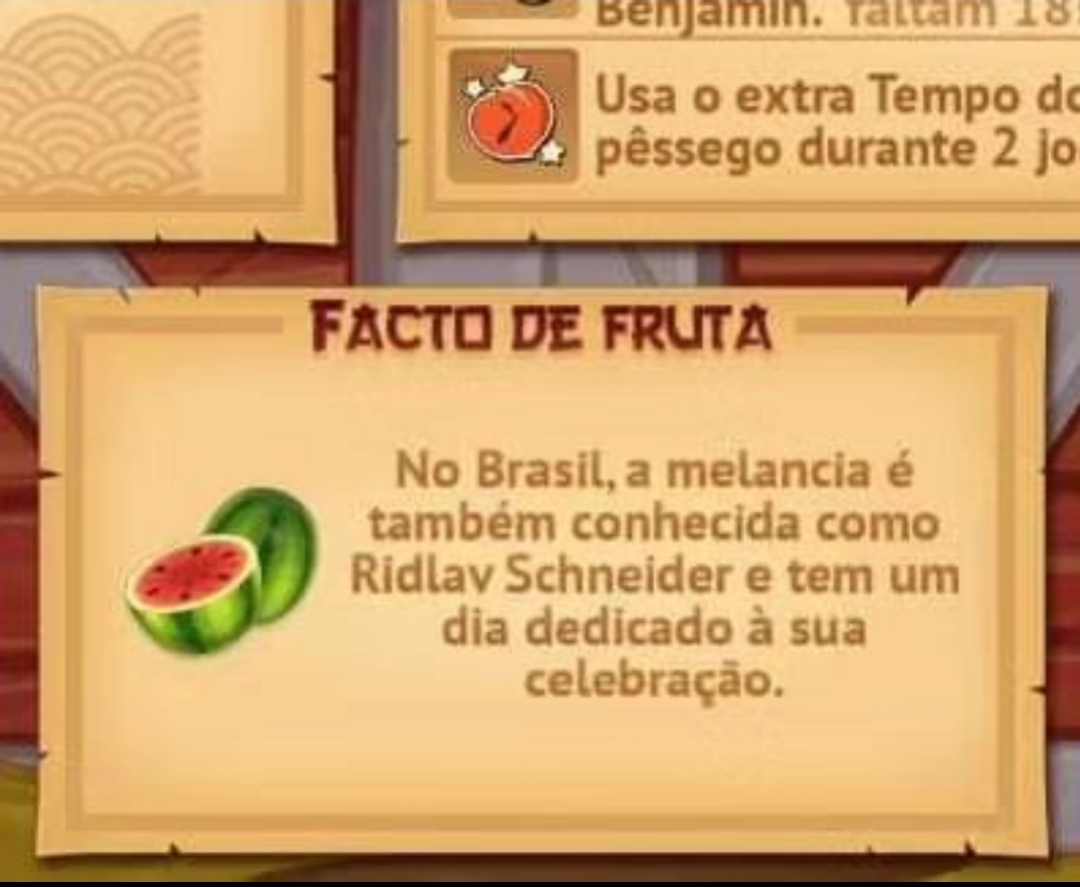
\includegraphics[width=1\linewidth]{pics/ridlavss.png}
    \caption{Fato mais desconhecido de todos os brasileiros.}
    \label{fig:ridlav}
\end{figure}


\begin{figure}[htb!]
    \centering
    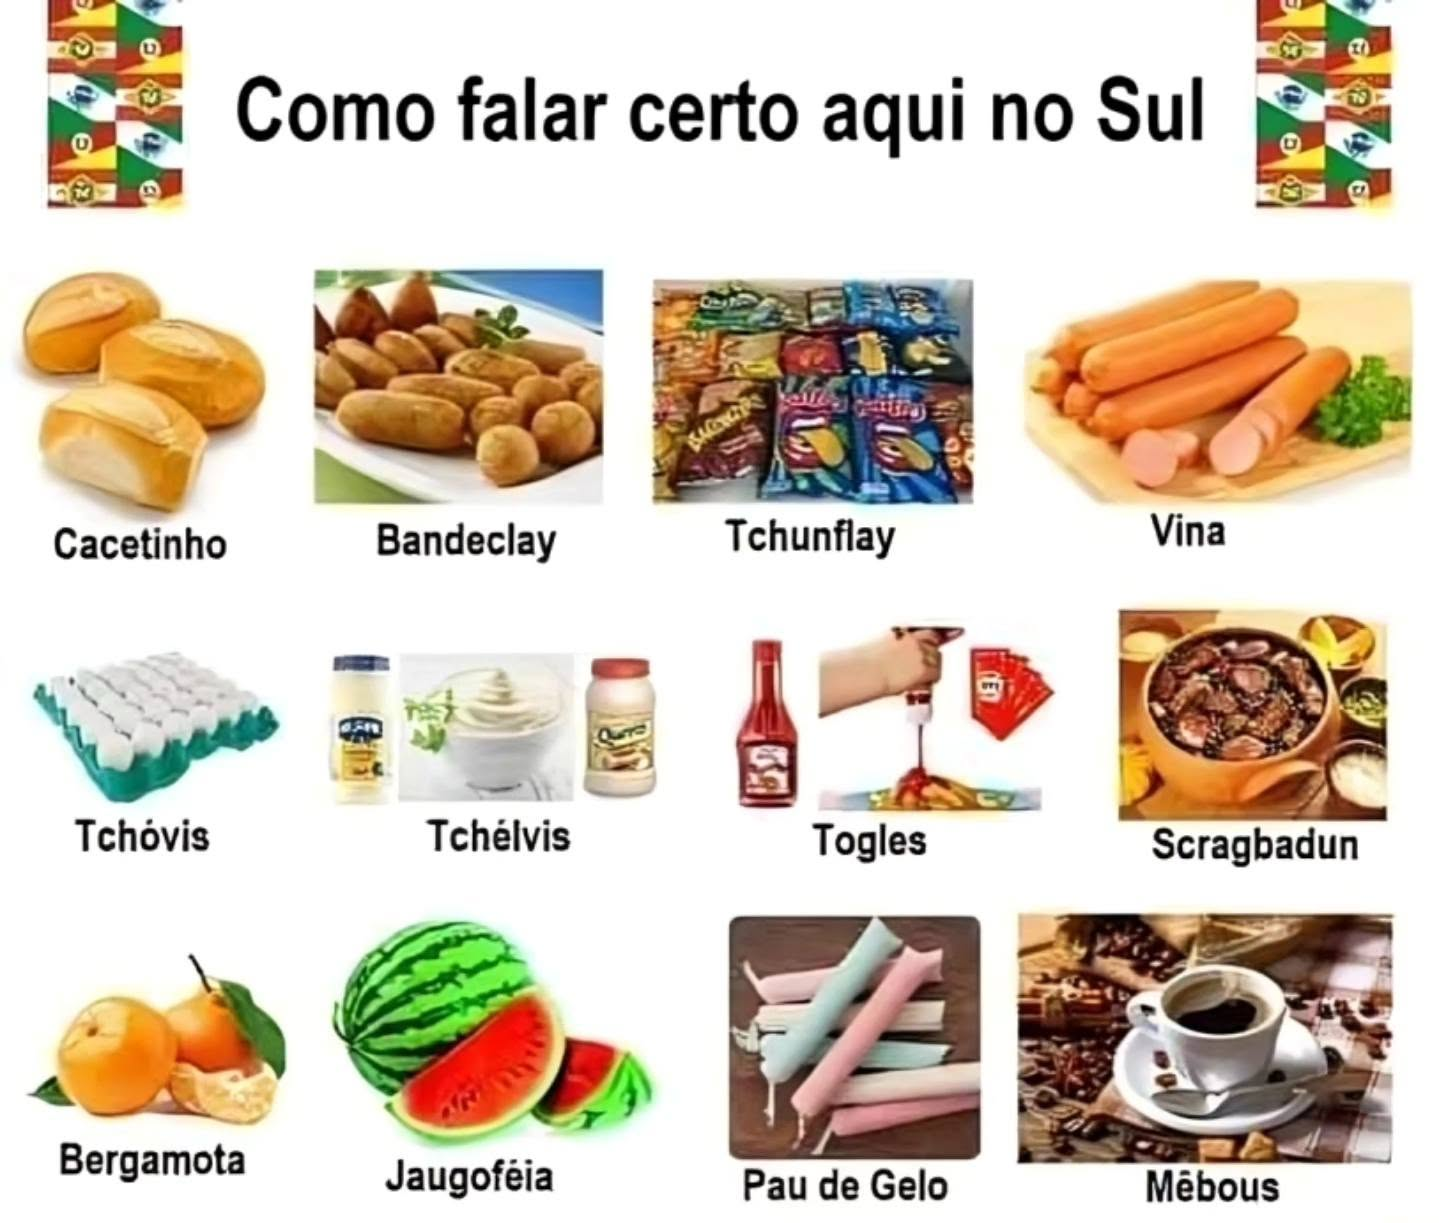
\includegraphics[width=1\linewidth]{pics/bandeclay.jpg}
    \caption{Mais informações supostamente desconhecidas.}
    \label{fig:bande}
\end{figure}

\begin{table}[htbp]
    \centering
    \caption{Componentes e seus valores}
    \begin{tabular}{lcr}
    \toprule
    Componente & Quantidade & Valor (R\$) \\
    \midrule
    Sensor Laser & 2 & 1500,00 \\
    Microcontrolador & 5 & 45,00 \\
    \bottomrule
\end{tabular}
\end{table}

\subsection{Aula 6}
A ideia foi aprender a fazer referências cruzadas e também referências bibliográficas. As referências cruzadas seriam aquelas citações que o autor faz de coisas que já estão dentro do corpo do texto, como uma imagem, tabela e por aí vai. Isso se faz com o uso dos labels específico de cada elemento no momento de sua inserção no texto. Caso ele tenha sido feito corretamente, a referência cruzada só chama essa informação do label para citação no texto.

Já as referências bibliográficas são aquelas que comumente aparecem no fim do documento, citando todas as fontes consultadas para elaboração da pesquisa. Pra essa o LaTeX faz uso de um arquivo externo, de extensão .bib. Uma vez configurado esse arquivo, é só incluir o comando de citação no corpo do texto que ele já puxa a referência indicada do arquivo .bib. É uma maravilha e funciona de uma forma que colabora muito mais pra manter a sanidade mental do autor do que ao utilizar o Word.

\subsection{Aula 7}
A aula de hoje foi sobre adaptação de templates acadêmicos. Até o momento utilizamos o template article, ele funciona bem pra rascunhos em geral, mas não compre com o que é necessário para trabalhos de publicação, por exemplo. É pra esse tipo de situação que abnTeX2 foi inventado. É um conjunto de ferramentas desenvolvidas por pesquisadores brasileiros que adapta o ambiente \LaTeX para redigir trabalhos no padrão ABNT. Dentro desse conjunto de ferramentas, temos suporte para comandos de folha de rosto, dedicatória, agradecimentos e até mesmo epígrafe, tudo formatado da maneira como deve ser. 

Um ponto interessante sobre revistas que aceitam publicações é a de que elas mesmas disponibilizam arquivos já configurados com o template exigido para qualquer um que queira submeter uma publicação. Esses arquivos de template devem ser colocados na mesma pasta onde os arquivos do trabalho em andamento se encontra e importados da devida forma no preâmbulo. Um ponto de atenção é o de resistir à tentação de simplesmente copiar e colar seco o arquivo redigido dentro de um que já utilize esse template. A chance de isso dar problema é bastante alta.

\subsection{Aula 8}
Chegou a hora de migrar do ambiente online do Overleaf para o local. Existem ambas vantagens e desvantagens ao fazer esta migração. Entre as vantagens estão a independência da conexão constante com a internet, o controle e acesso completo ao ambiente de desenvolvimento e a segurança de ter os dados em um local supostamente sem compartilhamento em rede.

Quanto às desvantagens podemos citar o fato de que a instalação local pode ser computacionalmente exigente em determinados casos, já que o pacote completo do LaTeX pesa por volta dos 15GB de armazenamento em disco. Outro ponto a ser destacado é a possível curva de aprendizado a ser manobrada pelo usuário na preparação do ambiente local. Como o Overleaf fazia muita coisa por conta própria por baixo dos panos, sem que o usuário tivesse a necessidade de pedir, aqui a coisa muda de figura. Por um lado é excelente que o usuário esteja totalmente no controle do ambiente, mas isso quer dizer que ele vai ter que saber exatamente o que está sendo executado e acontecendo dentro de seu próprio ambiente. Um ponto extra é a necessidade de se preocupar com seus arquivos, uma vez que não estão naturalmente armazenados com cópia na nuvem, mas somente de forma local, há uma camada extra de atenção para que eles não se percam para sempre por conta de eventuais falhas de hardware ou até mesmo deslizes do usuário.

De forma geral, o ambiente mais conveniente para se utilizar o LaTeX localmente é o VSCodium e suas variantes (blergh, VSCode aqui não). Além da instalação da extensão LaTeX Workshop, é preciso instalar o pŕoprio motor do LaTeX de forma separada, podendo o usuário optar pela instalação completa ()

\subsection{Aula 9}
\lipsum[1-2]

\subsection{Aula 10}
\lipsum[1]

\subsection{Aula 11}
\lipsum[1-2]

\subsection{Aula 12}
\lipsum[1]

\section{Considerações Finais}
\lipsum[1]


\bibliographystyle{plain}
\bibliography{ref}

\end{document} % Fecha o corpo do texto